\chapter{Конструкторская часть}

В этом разделе будут представлены требования к программному обес-
печению (ПО) и схема алгоритмов.

\section{Требования к программному обеспечению}

Программе передаются текст с орфографическими ошибками или без и словарь в качестве входных данных, а на выход получается текст без орфографических ошибок. Кроме того, необходимо сообщить пользователю затраченное каждым алгоритмом процессорное время.

В создаваемом приложении пользователю должен быть доступен выбор желаемого алгоритма.

\section{Разработка алгоритма поиска расстояния Левенштейна}

На рисунке~\ref{fig:levenstain} представлен алгоритм поиска расстояния Левенштейна.

\begin{figure}[h!]
	\centering{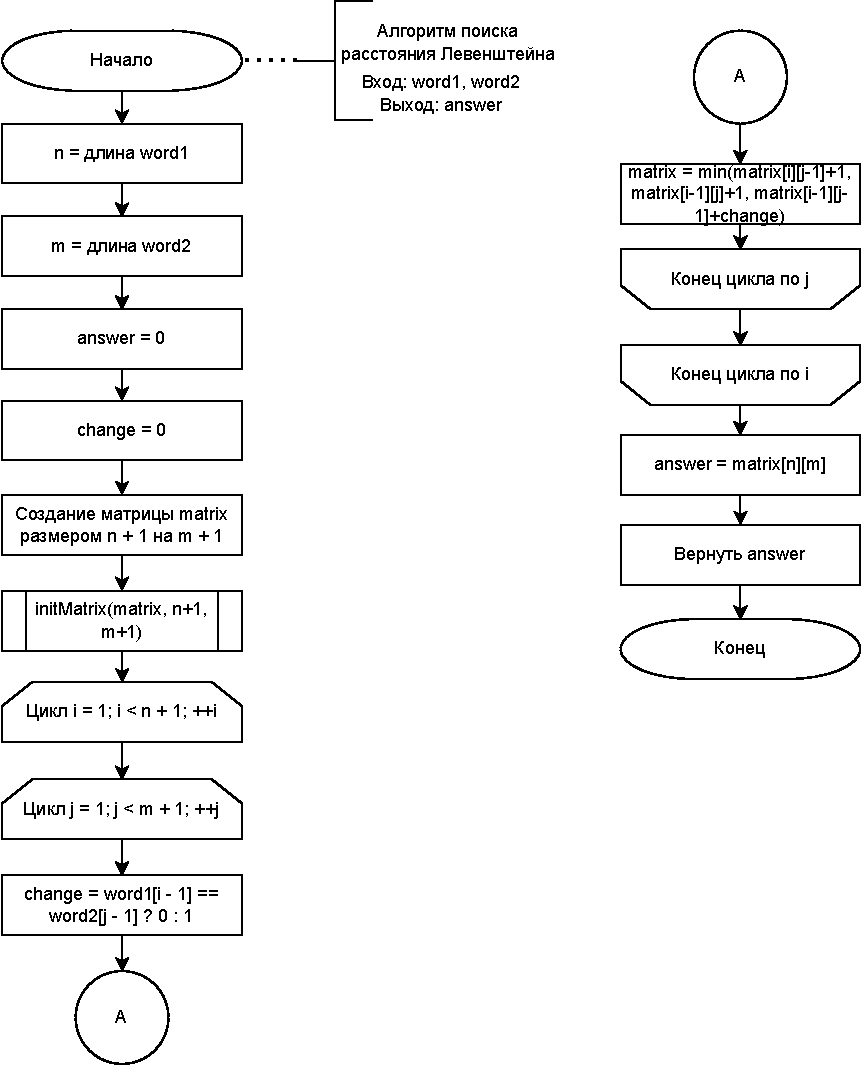
\includegraphics[scale=0.9]{photos/levenstain.pdf}}
	\caption{Алгоритм поиска расстояния Левенштейна}
	\label{fig:levenstain}
\end{figure}

\clearpage

\section{Разработка последовательного алгоритма}

На рисунке~\ref{fig:single_thread} представлен последовательный алгоритм.

\begin{figure}[h!]
	\centering{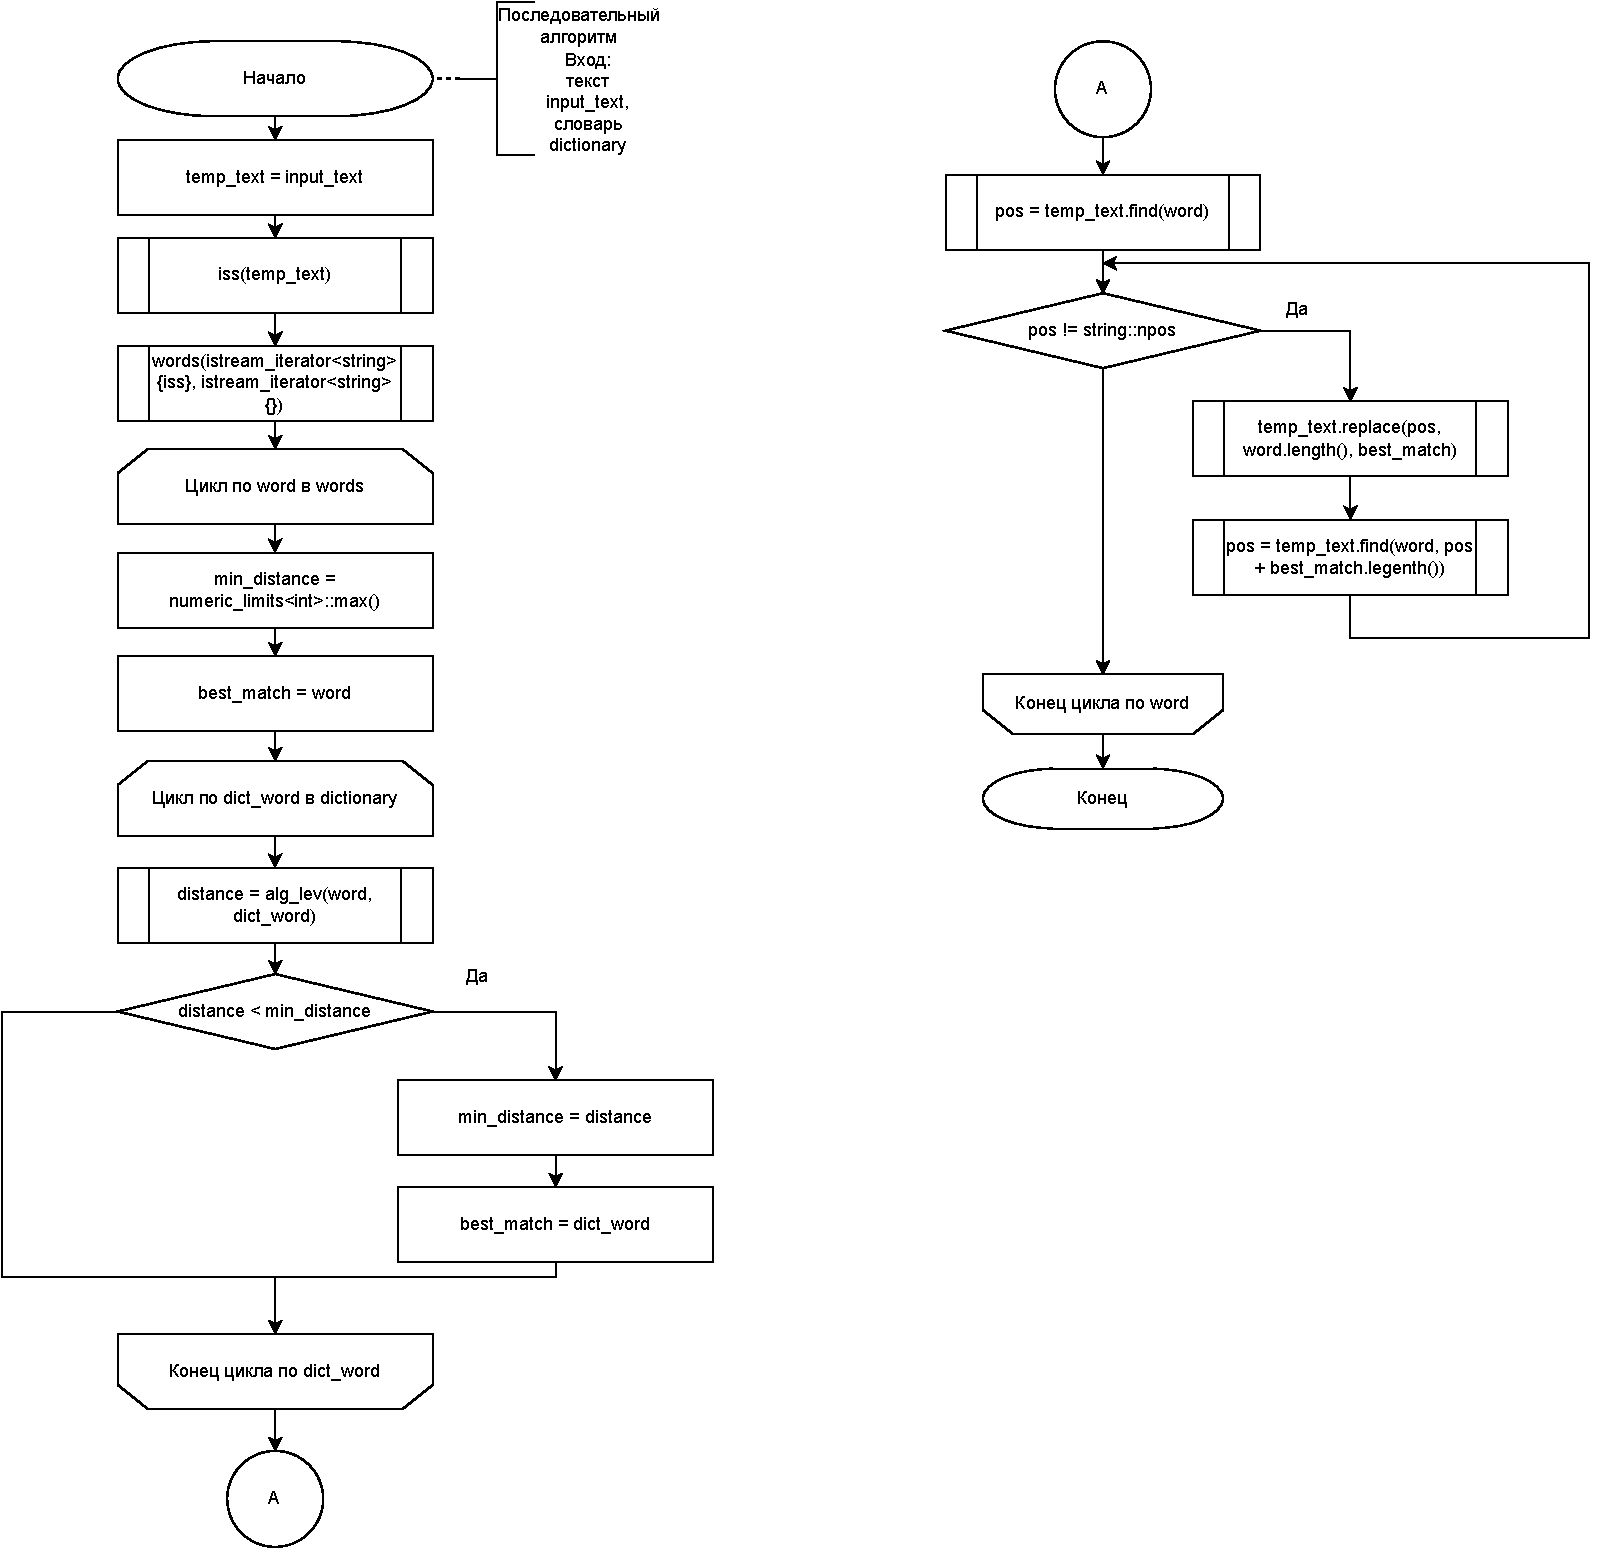
\includegraphics[scale=0.65]{photos/single_thread.pdf}}
	\caption{Последовательный алгоритм}
	\label{fig:single_thread}
\end{figure}

\clearpage

\section{Разработка многопоточного алгоритма}

На рисунке~\ref{fig:multi_thread} представлен многопоточный алгоритм.

\begin{figure}[h!]
	\centering{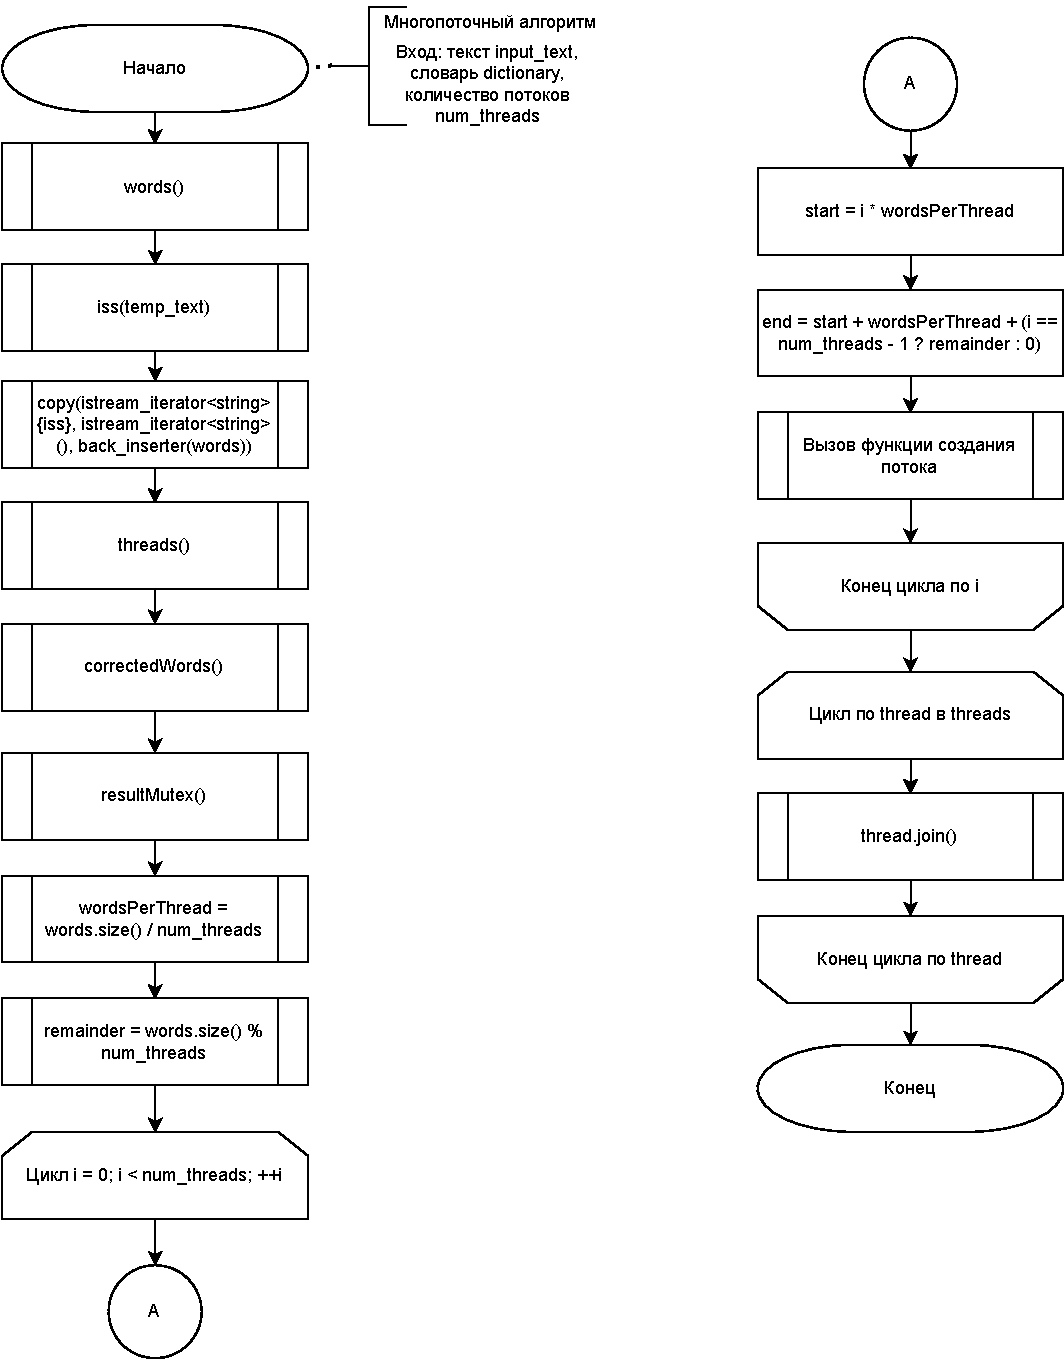
\includegraphics[scale=0.9]{photos/multi_thread.pdf}}
	\caption{Многопоточный алгоритм}
	\label{fig:multi_thread}
\end{figure}

\clearpage